\section{Facility Description}

\subsection{Location and Setting}

DreamLab is situated on a 5-acre plot in the Brecon Beacons vicinity, offering:

\begin{itemize}
    \item Strategic location: 30 minutes from Cardiff, 2 hours from Birmingham/Bristol
    \item Rural tranquillity with reliable infrastructure
    \item Stunning views and outdoor spaces for reflection and networking
    \item Direct access to walking trails and outdoor activities
    \item Secure, private setting ideal for focused learning
\end{itemize}

\subsection{AI Laboratory Specifications}

\subsubsection{Hardware Infrastructure}

\begin{labspec}
NVIDIA DGX A100 System & 8x A100 GPUs, 640GB GPU memory & 1 & \pounds{150,000} \\
GPU Workstations & RTX 4090, 64GB RAM, 2TB NVMe & 12 & \pounds{60,000} \\
Edge Computing Kit & Jetson Orin development boards & 20 & \pounds{15,000} \\
Network Infrastructure & 10Gb switches, enterprise firewall & 1 set & \pounds{25,000} \\
Storage Server & 200TB RAID array, backup system & 1 & \pounds{20,000} \\
\end{labspec}

\subsubsection{Software and Licenses}

\begin{itemize}
    \item NVIDIA AI Enterprise Suite
    \item Microsoft Azure credits (\pounds{50,000} annual partnership)
    \item AWS educate programme access
    \item Open-source ML frameworks (TensorFlow, PyTorch, JAX)
    \item Custom DreamLab learning management system
\end{itemize}

\subsubsection{Laboratory Layout}

\begin{center}
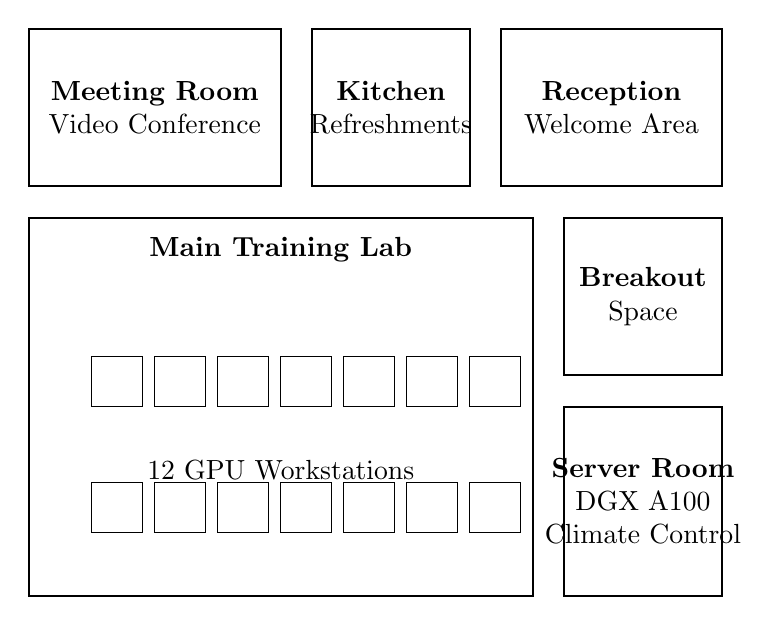
\begin{tikzpicture}[scale=0.8]
    % Main lab
    \draw[thick] (0,0) rectangle (8,6);
    \node at (4,5.5) {\textbf{Main Training Lab}};
    
    % Workstations
    \foreach \x in {1,2,3,4,5,6,7}
    \foreach \y in {1,3}
    {
        \draw (\x,\y) rectangle (\x+0.8,\y+0.8);
    }
    \node at (4,2) {12 GPU Workstations};
    
    % Server room
    \draw[thick] (8.5,0) rectangle (11,3);
    \node[align=center] at (9.75,1.5) {\textbf{Server Room}\\DGX A100\\Climate Control};
    
    % Breakout space
    \draw[thick] (8.5,3.5) rectangle (11,6);
    \node[align=center] at (9.75,4.75) {\textbf{Breakout}\\Space};
    
    % Meeting room
    \draw[thick] (0,6.5) rectangle (4,9);
    \node[align=center] at (2,7.75) {\textbf{Meeting Room}\\Video Conference};
    
    % Kitchen
    \draw[thick] (4.5,6.5) rectangle (7,9);
    \node[align=center] at (5.75,7.75) {\textbf{Kitchen}\\Refreshments};
    
    % Reception
    \draw[thick] (7.5,6.5) rectangle (11,9);
    \node[align=center] at (9.25,7.75) {\textbf{Reception}\\Welcome Area};
\end{tikzpicture}
\end{center}

\subsection{Accommodation Features}

\subsubsection{Main Residence}

A beautifully renovated 4-bedroom Welsh farmhouse featuring:

\begin{itemize}
    \item \textbf{Bedrooms}: 4 ensuite rooms, sleeps 8-10 comfortably
    \item \textbf{Living Spaces}: Open-plan kitchen/dining, two lounges, study
    \item \textbf{Business Facilities}: Dedicated office space, video conferencing setup
    \item \textbf{Wellness}: Hot tub, sauna, exercise room
    \item \textbf{Outdoor}: Large patio, BBQ area, gardens
\end{itemize}

\subsubsection{Sustainable Features}

\begin{solarroi}
\textbf{12kW Solar Installation with Battery Storage}

\begin{table}[H]
\centering
\begin{tabular}{lr}
\toprule
\textbf{Component} & \textbf{Specification} \\
\midrule
Solar Panels & 30x 400W panels (12kW total) \\
Battery Storage & 3x Tesla Powerwall (40.5kWh) \\
Annual Generation & 11,000 kWh estimated \\
Grid Independence & 70-80\% average \\
Payback Period & 6-7 years \\
25-year Savings & \pounds{125,000} projected \\
\bottomrule
\end{tabular}
\end{table}
\end{solarroi}

\subsubsection{EV Infrastructure}

\begin{itemize}
    \item 2x Tesla Wall Connectors (11kW)
    \item 2x Universal Type 2 chargers (7kW)
    \item Solar-powered charging capability
    \item Guest booking system integration
\end{itemize}

\subsection{Phased Development Plan}

\begin{center}
\phasedtimeline{
    \gantttitle{Development Timeline}{12} \\
    \gantttitlelist{1,...,12}{1} \\
    \ganttgroup{Phase 1: Core Lab}{1}{4} \\
    \ganttbar{Lab Construction}{1}{3} \\
    \ganttbar{Equipment Install}{3}{4} \\
    \ganttmilestone{Lab Operational}{4} \\
    \ganttgroup{Phase 2: Accommodation}{4}{8} \\
    \ganttbar{Renovation}{4}{7} \\
    \ganttbar{Furnishing}{7}{8} \\
    \ganttmilestone{Letting Ready}{8} \\
    \ganttgroup{Phase 3: Sustainability}{8}{12} \\
    \ganttbar{Solar Installation}{8}{10} \\
    \ganttbar{EV Charging}{10}{11} \\
    \ganttbar{Landscaping}{10}{12} \\
    \ganttmilestone{Fully Operational}{12}
}
\end{center}

\subsection{Accessibility and Inclusivity}

DreamLab is committed to being fully accessible:

\begin{itemize}
    \item Ground-floor training facilities with wheelchair access
    \item Accessible accommodation room available
    \item Hearing loop systems in all training areas
    \item Height-adjustable workstations
    \item Assistive technology software available
\end{itemize}

\subsection{Security and Safety}

\begin{itemize}
    \item 24/7 CCTV monitoring of lab facilities
    \item Biometric access control to server room
    \item Fire suppression system in all areas
    \item First aid trained staff on-site
    \item Comprehensive insurance coverage
    \item Data security: ISO 27001 compliance planned
\end{itemize}